\section{Case study: \acf{AV} braking}
\label{sec:case}

\acfp{AV} are \acfp{CPS} that are safety critical: any faults in their operation can lead to accidents resulting in injuries or fatalities; such as Tesla's and Uber's accidents~\cite{coldewey_2018}~\cite{stewart_2018}.
In this chapter, we take inspiration from such accidents and create a case study involving the braking mechanism of \acp{AV}.

We propose a abstract \acf{AV} represented in Figure~\ref{fig:av}.
We deal with the linear, forward movement of the \ac{AV} and the braking involved with such movement.

\begin{figure}[h]
	\centering
	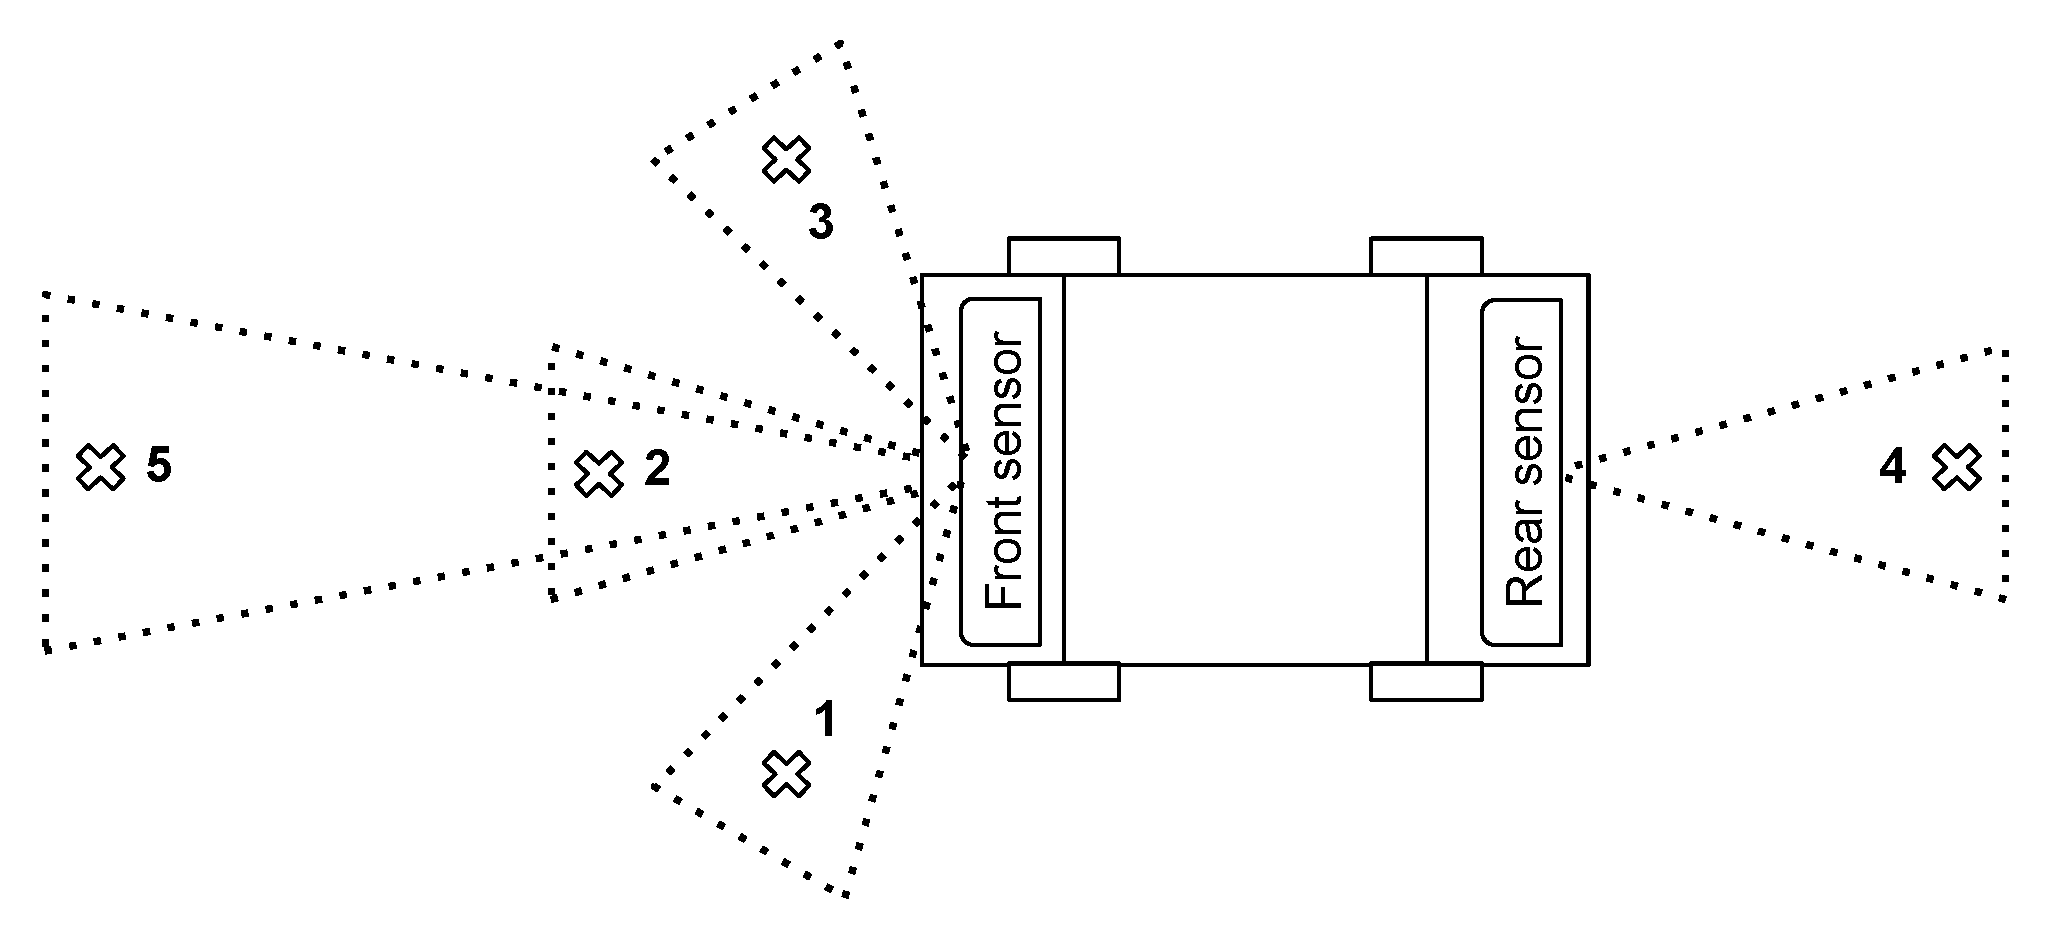
\includegraphics[width=\textwidth]{Content/fig/AV.pdf}
	\caption{Sensor layout for the \ac{AV} example. \label{fig:av}}
\end{figure}

\subsection{\acf{AV} system}
The \ac{AV} system used in this chapter consists of on vehicle, run by an autonomous controller, with 5 directional, sensor inputs (see Figure~\ref{fig:av}).
The sensor package consists of five cameras, each with its own, unique field of view and a \acf{LiDAR} sensor.
Each camera picks up a certain area in the surrounding area, and each camera has an associated \ac{LiDAR} reading for the area is is detecting.
Each of the five cameras feeds into a \acf{MNN} ensemble~\cite{Maqsood2004} of \acp{SNN}, using the Darknet library~\cite{darknet13}, while the \ac{LiDAR} reading are passed directly to the controller.
These ensembles will be covered in the \ac{AI} section of this case study.
These \ac{SNN} ensembles classify their input image and provide a confidence level for the classified image, before passing this information to the controller.
The controller \ac{SNN} is a \ac{MLP}, and decides the best course of action given the environment and the status of the vehicle itself. 
The current status of the vehicle is noted by the current speed of the vehicle ($S$) and the previous speed of the vehicle($S'$).
The controller then outputs one of three simple commands to the vehicles actuators which are represented by an accelerator and a brake.
These commands are as follows: accelerate ($A$); brake softly ($B_S$); and brake hard ($B_H$).
A block diagram of the \ac{AV} used in this system is shown in Figure~\ref{fig:avnenf}. 

\begin{figure}[h]
	\centering
	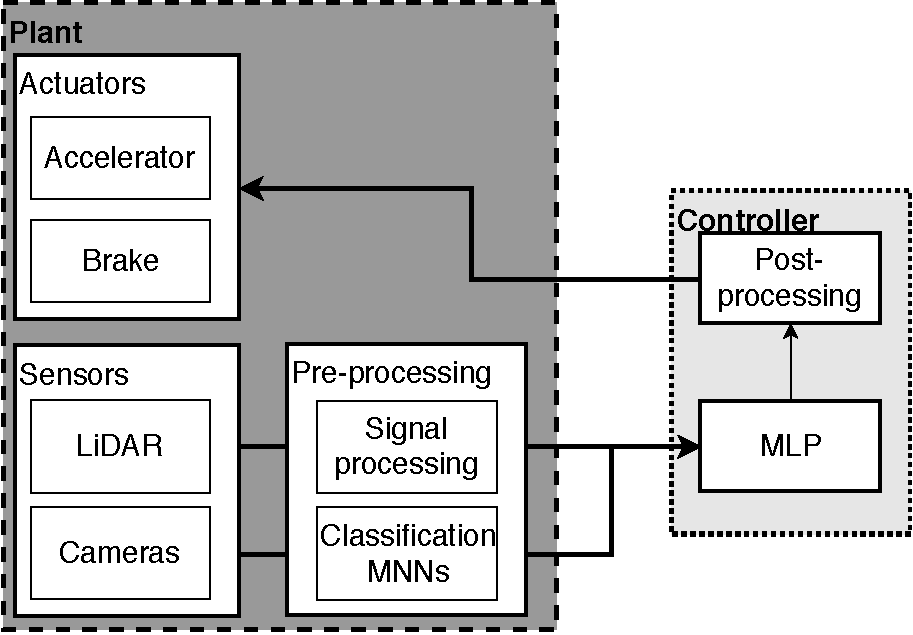
\includegraphics[width=\textwidth]{Content/fig/AV-sys-nenf.pdf}
	\caption{Block diagram of the \ac{AV} system used in the case study. \label{fig:avnenf}}
\end{figure}

The system controller, \acp{MNN} and sensor readings are all synchronous and, as such, the system is run using synchronous semantics.
The synchronous language Esterel is used to run the entirety of the system controller and its connected components.
The entire system is run in two logical clock cycles; a single cycle for the plant and a single cycle for the controller \ac{MLP}.
The \ac{MNN} ensembles are run concurrently with each other, followed by the execution of the controller \ac{MLP} on the \ac{MNN} ensembles' outputs.
The environment update is run in the same cycle as the sensor readings and plant execution, with the environment updating before new sensor readings are taken.

The environment for this \ac{AV} system consists of the \ac{AV} in question, and up to five other ``objects'' ($O$) in the environment.
Each sensor position in the \ac{AV} system (Figure~\ref{fig:av}) can detect up to one object at that position at any one time, represented by the numbered position at which the object was detected.
Each object can be a person ($P~=~0$), a car ($C~=~1$) or nothing ($N~=~3$).
Each object detected by a camera is represented by the sensor position it is detected in and the type of object it is.
E.g. an person behind the vehicle would be $O_{4}~=~0$, a vehicle directly in front would be $O_{2}~=~1$ and nothing to the right side of the \ac{AV} would be $O_{3}~=~N$.
Each object additionally has a speed and direction assigned to it: $O_{5_S}$ refers to the speed of the object far ahead; $O_{1_D}$ refers to the direction of the object to the left of the vehicle.
The system used three possible speeds (stationary, slow, fast) represented by an integer value (0, 1, 2) respectively.
The directions were limited to (North, East, South and West), represented by the numerical values (0, 1, 2 and 3) respectively.

The environment updated in such a way that objects would move in the direction they are facing at a speed relative to the \ac{AV}.
For example, a pedestrian facing the road and moving quickly would be placed in front of the vehicle in position 2 on the next clock cycle.
However, a pedestrian moving away from the road, or not moving at all, would be removed from the sensors detection areas on the next clock cycle.
Each update cycle, each camera ``produced'' an appropriate input image from the \ac{VOC} 2012 dataset~\cite{pascal-voc-2012} as the object in that position (either a person, car or nothing).

Due to this design of this system, it is possible for the vehicle to behave badly in various ways. 
These include speeding, unnecessarily braking, hitting other vehicles on the road, hitting pedestrians on the road and even not driving at all.
All of these scenarios can result in fatalities, thus classifying this system as a safety critical.
To have a system that is safe, policies need to be enforced that monitor the system's inputs and outputs and ensure that none of the above scenarios take place under any circumstances.

\subsection{Run-time enforcer for the \acf{AV} system}
We propose the use of a run-time enforcer~\cite{recps} between the plant and controller (see Figure~\ref{fig:avenf}), to provide formal guarantees about the controller \ac{SNN}'s functional safety.
This enforcer will monitor the I/O events of the controller \ac{SNN} and \textit{edit} unsafe events so that controller functions safely.

\begin{figure}[h]
	\centering
	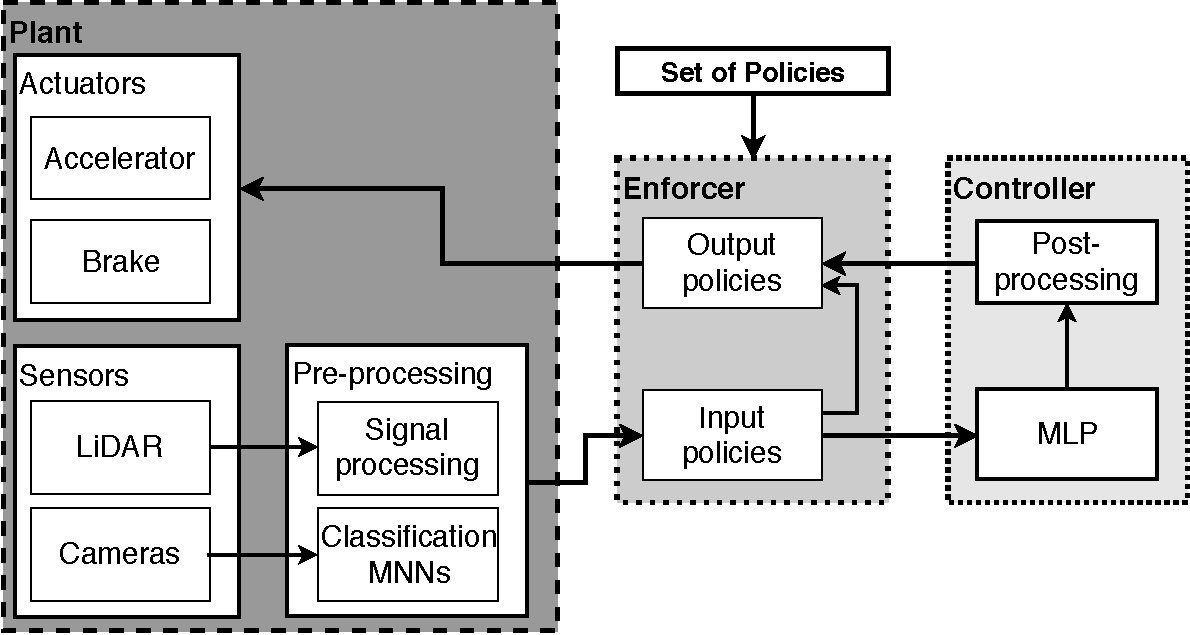
\includegraphics[width=\textwidth]{Content/fig/AV-sys.pdf}
	\caption{Block diagram of the \ac{AV} system, with run-time enforcer, used in the case study. \label{fig:avenf}}
\end{figure}

\subsection{\acf{AI} for the \acf{AV} system}

The \acp{AI} in this case study include the \ac{MMN} ensembles in the plant and a single \ac{MLP} \ac{SNN} for the controller.

An \ac{ANN} ensemble the parallel execution of multiple \acp{ANN} working in combination to produce more accurate output~\cite{Maqsood2004}.
In this case study, each \ac{MNN} consisted of three \acp{CNN}.
Each \ac{CNN} in the ensemble provided its output to an ensemble function, which then produced higher grade output using a custom averaging function based off the \acp{CNN}' class scores.
Due to the synchronous nature of the \acp{CNN}, each \ac{CNN} was run in synchronous concurrency with the others to provide output to the ensemble function.
	
Each \ac{CNN} consists of 10 layers: a combination of convolutional, maximum pooling and average pooling layers.
Each \ac{CNN} was trained for up to 100,000 epochs on the \acf{VOC} 2012 data set, using the Darknet C library~\cite{darknet13} to perform back-propagation with gradient descent.
The \acp{CNN} took an input image of 28x28 pixels and output three class probabilities; one for a person, one for a car and one for nothing.

The controller \ac{MLP} consisted of three layers of artificial neurons, with seventeen input neurons, ten hidden layer neurons and three output neurons.
The implemented system and environment were complex enough that back-propagation was not an applicable method to train the controller, as the desired outputs for a set of seventeen different inputs was not possible effectively map by hand.
The controller \ac{MLP} was trained used a type of reinforcement learning called Q-learning~\cite{qlearning2010}.
This training processes works by reinforcing good actions with positive rewards, and removing bad actions with negative rewards.
Like the \acp{CNN}, this ac{ANN} was also trained for up to 100,000 epochs using this technique.
The controller took the seventeen different inputs, as an array of integers, in the following order (using the previously defined labels): $(S, S', O_1, O_2, O_3, O_4, O_5, O_{1_D}, O_{2_D}, O_{3_D}, O_{4_D}, O_{5_D}, O_{1_S}, O_{2_S}, O_{3_S}, O_{4_S}, O_{5_S})$.
The outputs of the controller were a binary array representing the actions that could be taken: $(A, B_S, B_H)$, where each value could be $1$ or $0$.

Figure~\ref{fig:avmnn} is an expanded diagram of the \ac{AV} system, showing the \ac{ANN} layout for this system.
Each \ac{MNN} ensemble is labelled by its corresponding sensor number and shows three \acp{CNN} feeding into a single ensemble function for each \ac{MNN}.
The ensemble outputs are then passed to the controller \ac{SNN} \ac{MLP} via the input run-time enforcer.
The controller's decision is made by its \ac{MLP}, and then passed back to the vehicle via the output enforcer.

\begin{figure}[H]
	\centering
	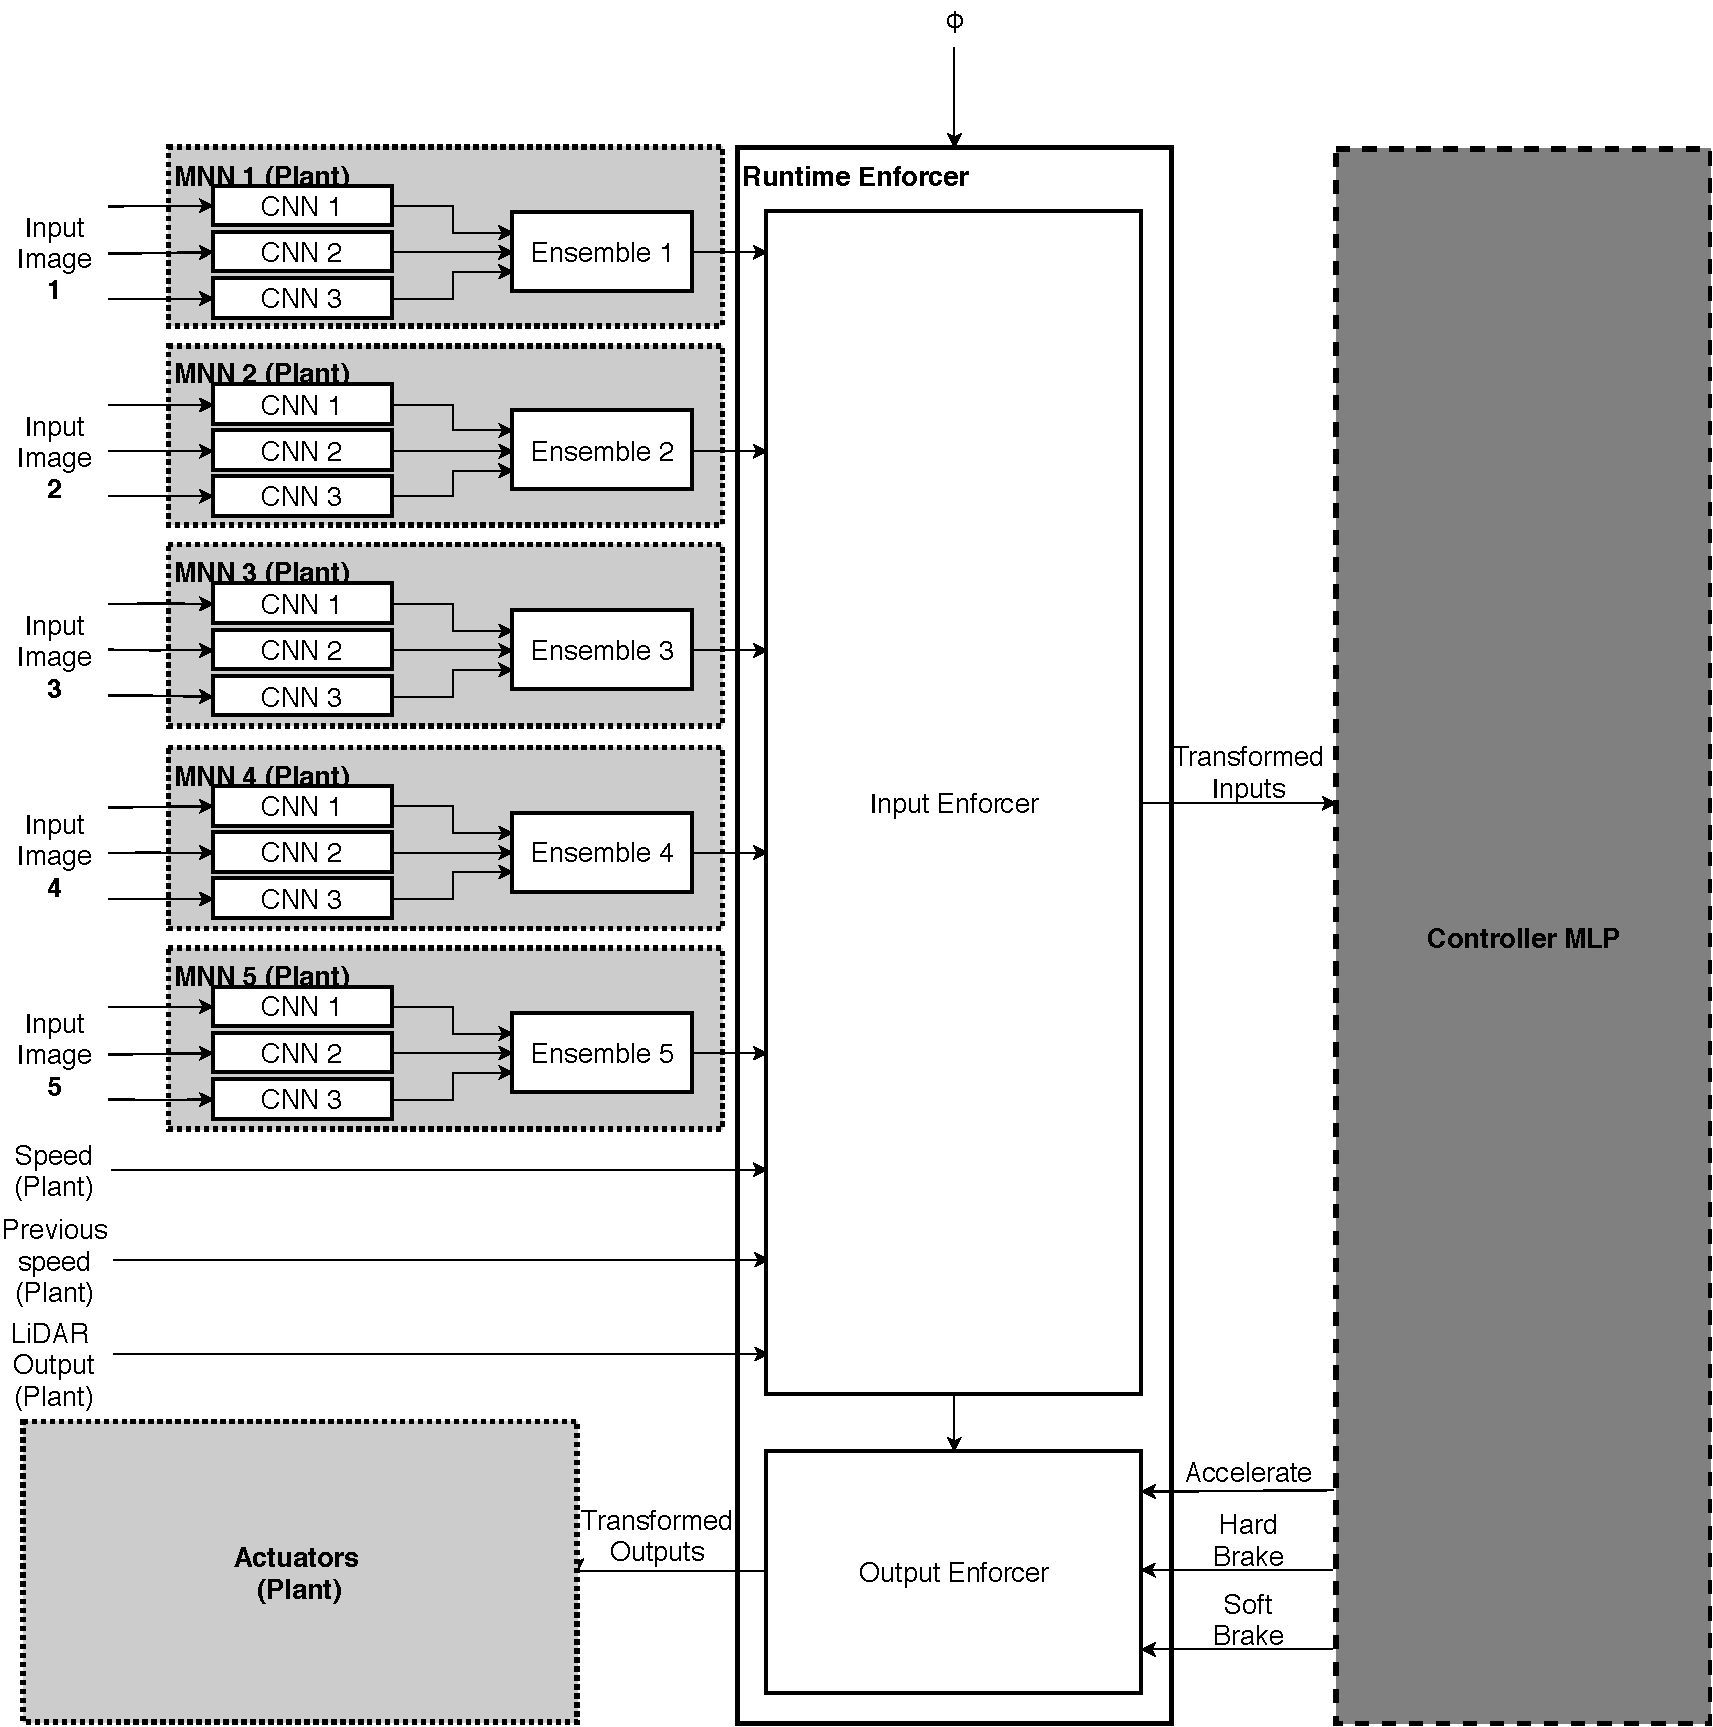
\includegraphics[width=\textwidth]{Content/fig/AV-MNN.pdf}
	\caption{Diagram showing the \ac{SNN} for the \ac{AV}, and its interaction with the plant via the enforcer. \label{fig:avmnn}}
\end{figure}



